\documentclass[9pt]{extarticle}

\usepackage[utf8]{inputenc}
\usepackage[T1]{fontenc}
\usepackage{lmodern}
\usepackage{graphicx}
\usepackage{color}
\usepackage{hyperref}
\usepackage{amsmath}
\usepackage{amsfonts}
\usepackage{epstopdf}
\usepackage[table]{xcolor}
\usepackage[a4paper, total={6in, 10in}]{geometry}
\usepackage{enumitem}
\usepackage[export]{adjustbox}


\graphicspath{ {./Figures/} }


\begin{document}

{\huge Andrew Sivaprakasam | Cochlear Implant Project 2020 Write-up}
\begin{center}
GitHub Repo: \url{https://github.com/sivaprakasaman/511_Cochlear_Implant_Project}
\end{center}

\section{Part A | Introduction to cochlear-implant signal processing}

\begin{enumerate}[label = \alph*) ]
\item Filter-bank reconstructions were generated using the \verb|quad_filt_bank.m| function from Delgutte within the \verb|get_Stimuli.m| function I created. The bands were set using the \verb|equal_xbm_bands.m| function from Delgutte. This function spaced the frequency bands to match the frequency distribution of the basilar membrane using Liberman's cat cochlear frequency map, scaling it to match the \textasciitilde 20 kHz hearing range of humans. For cochlear implant user simulation, this is important, since we assume cochlear implant electrodes are equally spaced. However, the frequency-specific IHCs in the cochlea are not equally spaced from 0-4 kHz, so this correction accounts for this.  

\vspace{.5em}

Refer to \verb|B| in my \verb|get_Stimuli.m| code for the filter coefficients. 

\item Below are the different envelope extractions visualized for the 1 band filter-bank. It is apparent that the Hilbert envelope is more thorough than the 16 and 160 Hz envelope extraction methods, allowing it to capture a more detailed picture of amplitude variations in the sound being played. 

\begin{center}
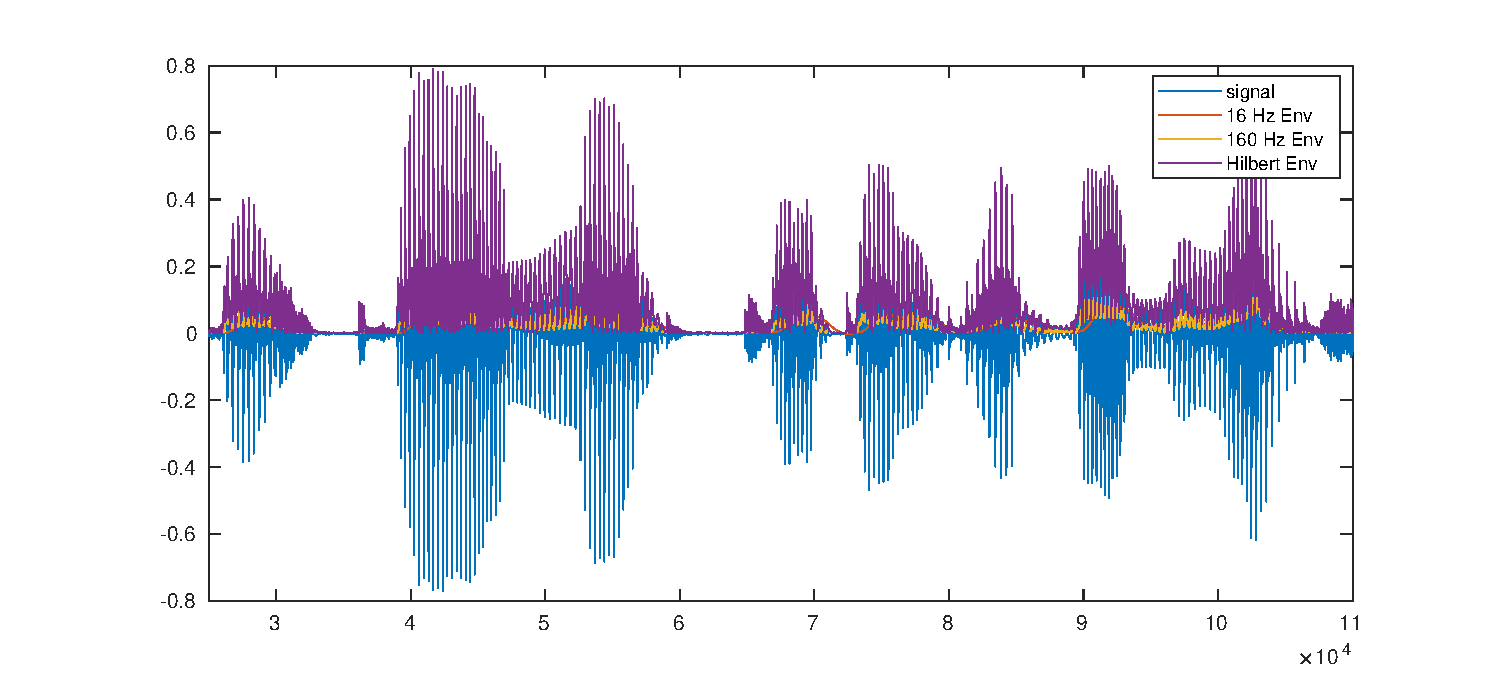
\includegraphics[width = .85\textwidth]{envelopes}
\end{center}

\item Here are some spectrograms (bandwidth 30 Hz, dynamic range 45 dB) that demonstrate proof of a working filter-bank: \\

\hspace{6.5em}\textbf{16 Hz} \hspace{11em} \textbf{160 Hz} \hspace{9em} \textbf{Hilbert}

\begin{center}
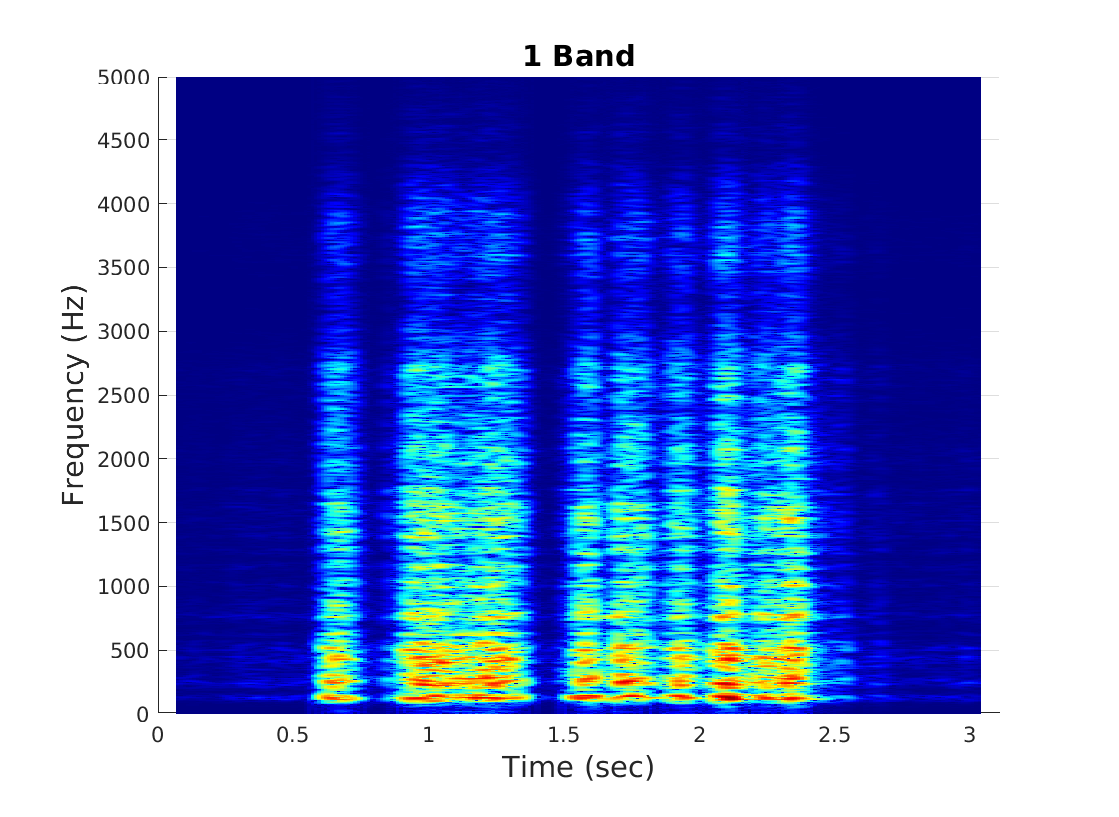
\includegraphics[width = .3\textwidth]{16_1}
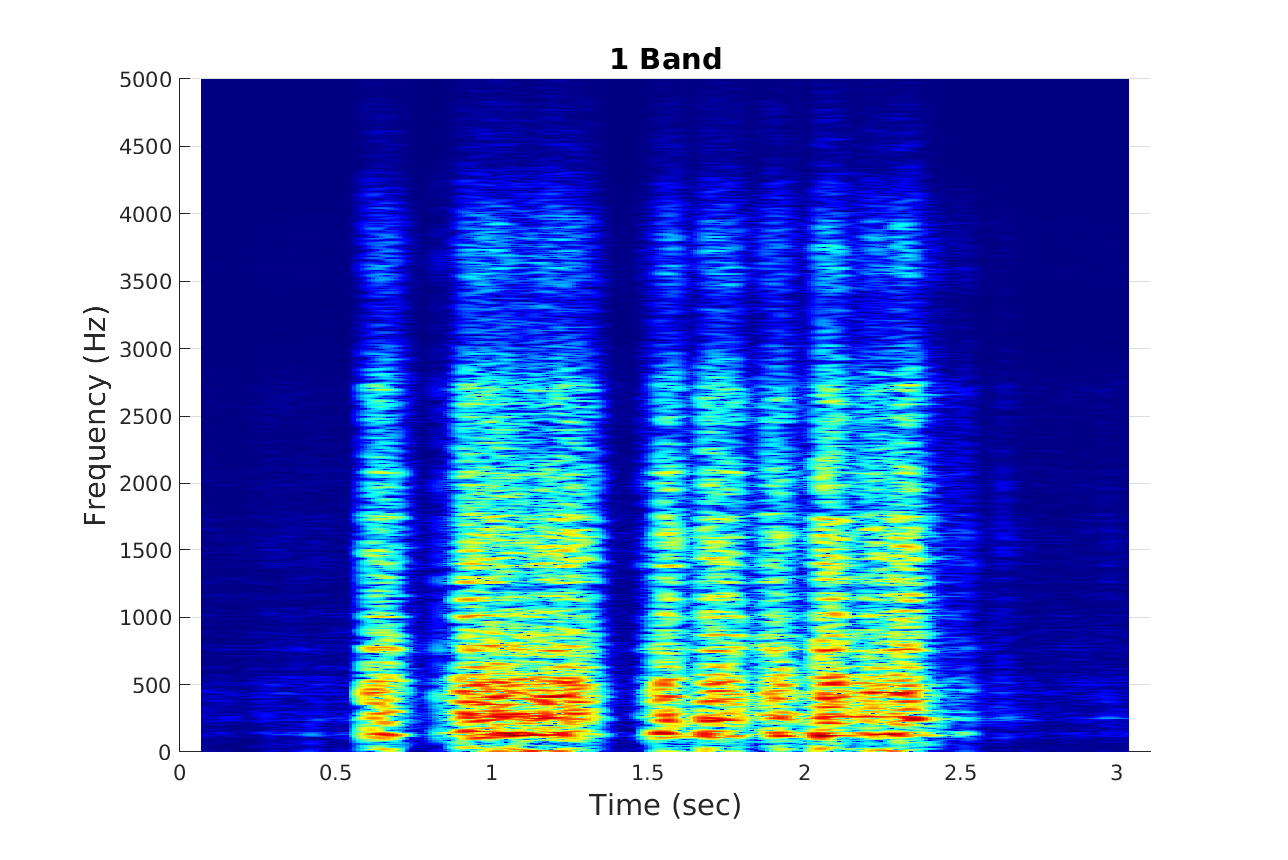
\includegraphics[width = .3\textwidth]{160_1}
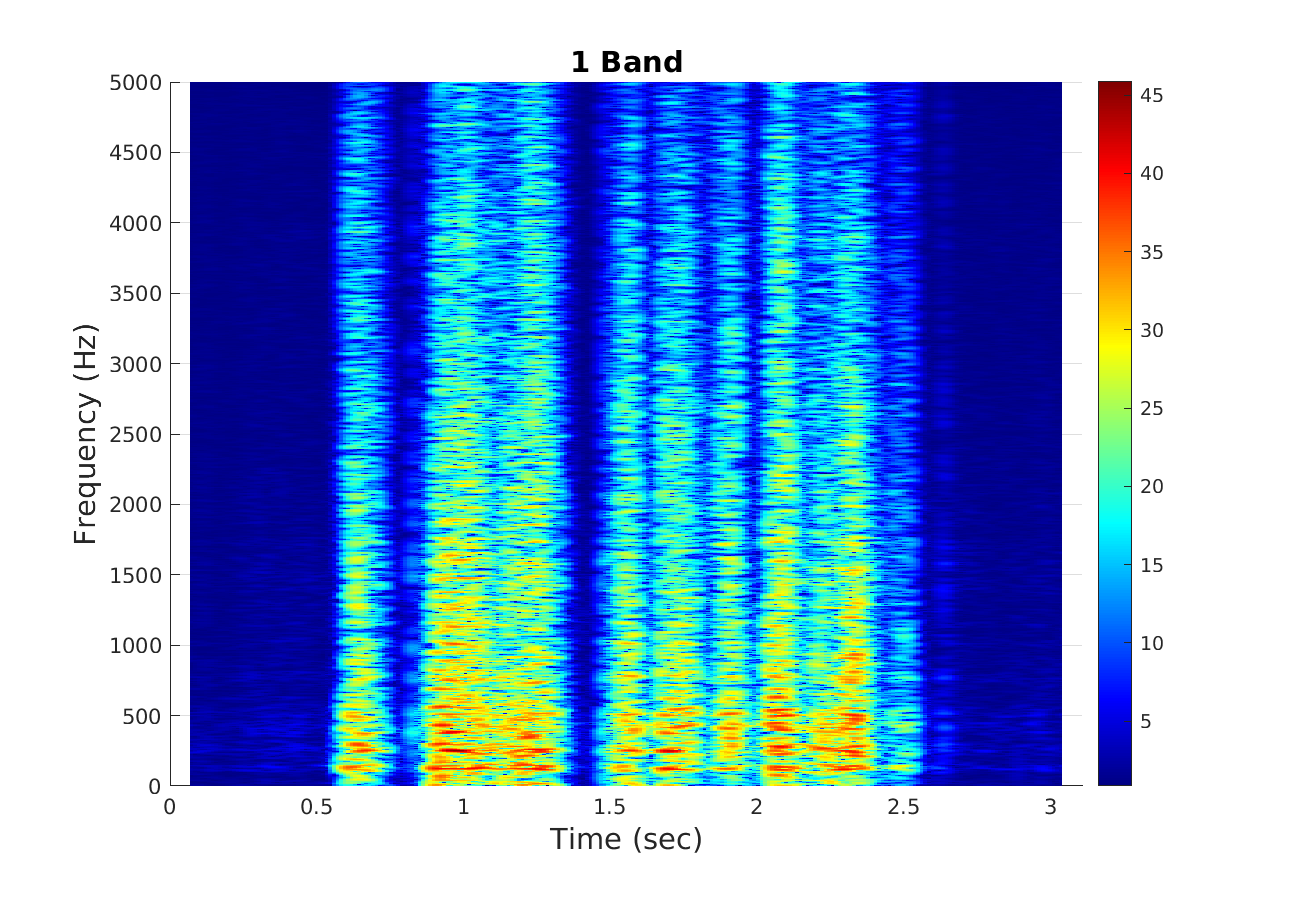
\includegraphics[width = .3\textwidth]{hilb_1} \\

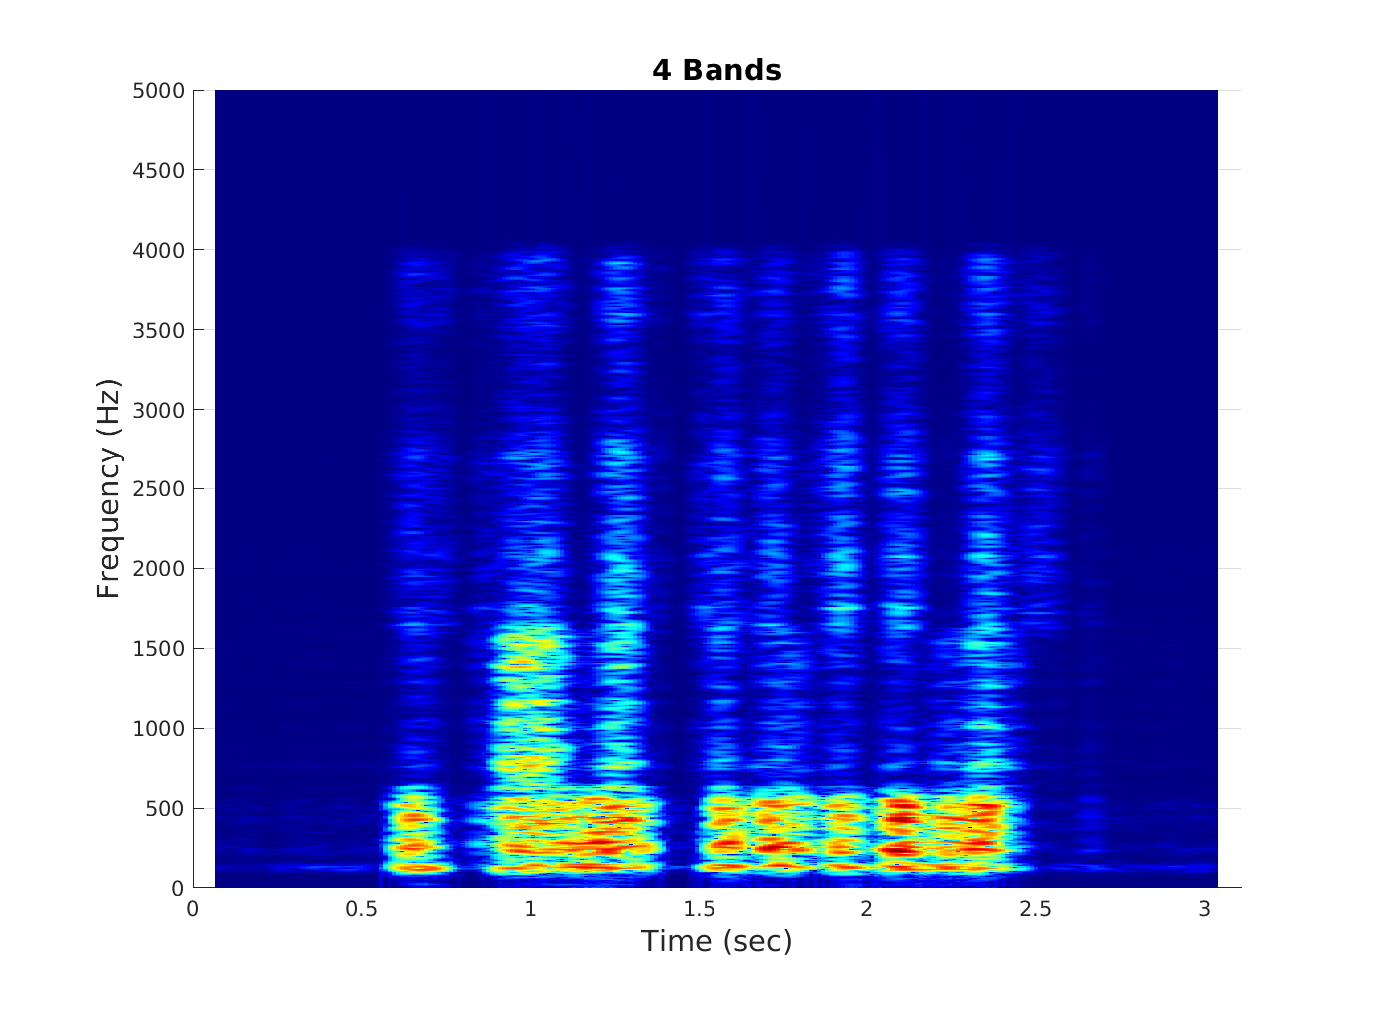
\includegraphics[width = .3\textwidth]{16_4}
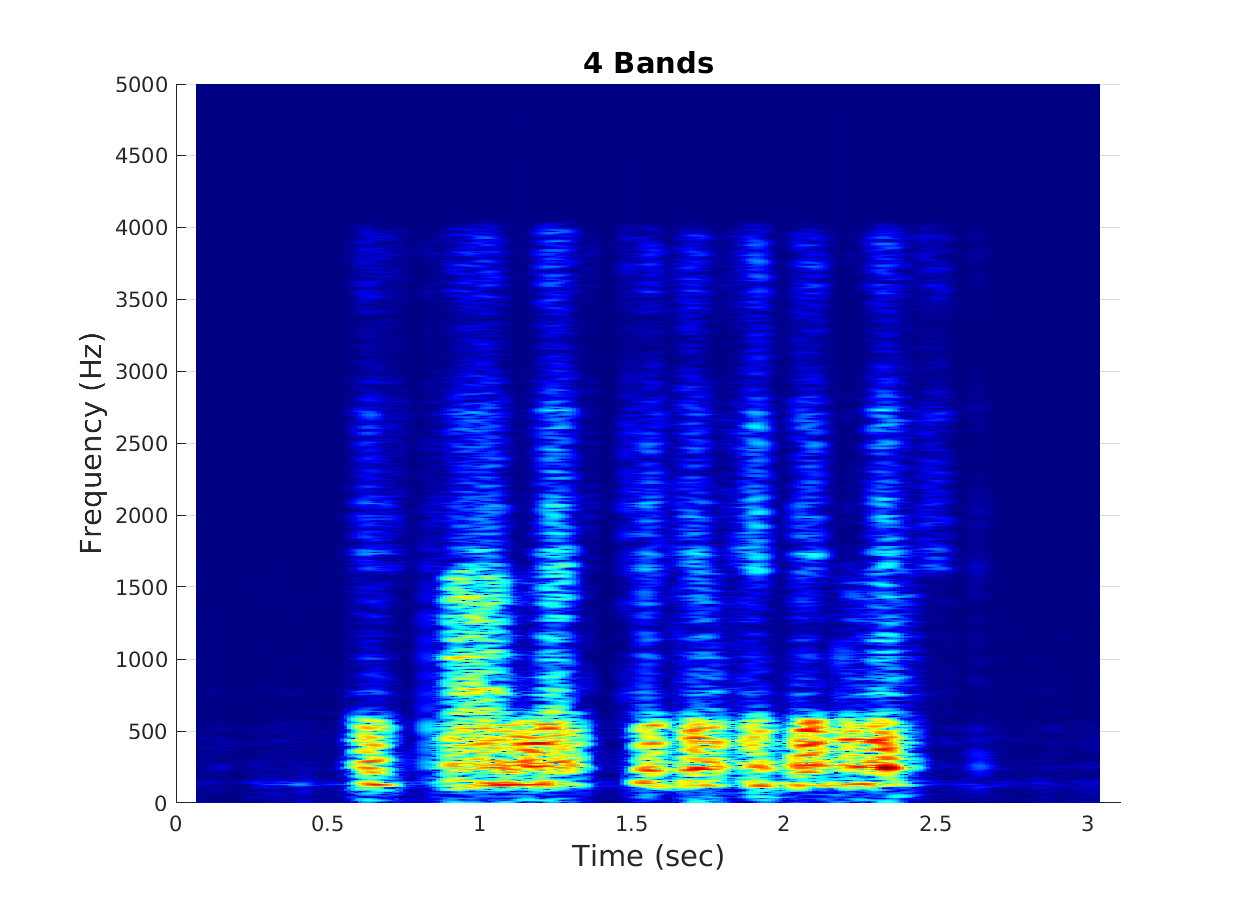
\includegraphics[width = .3\textwidth]{160_4}
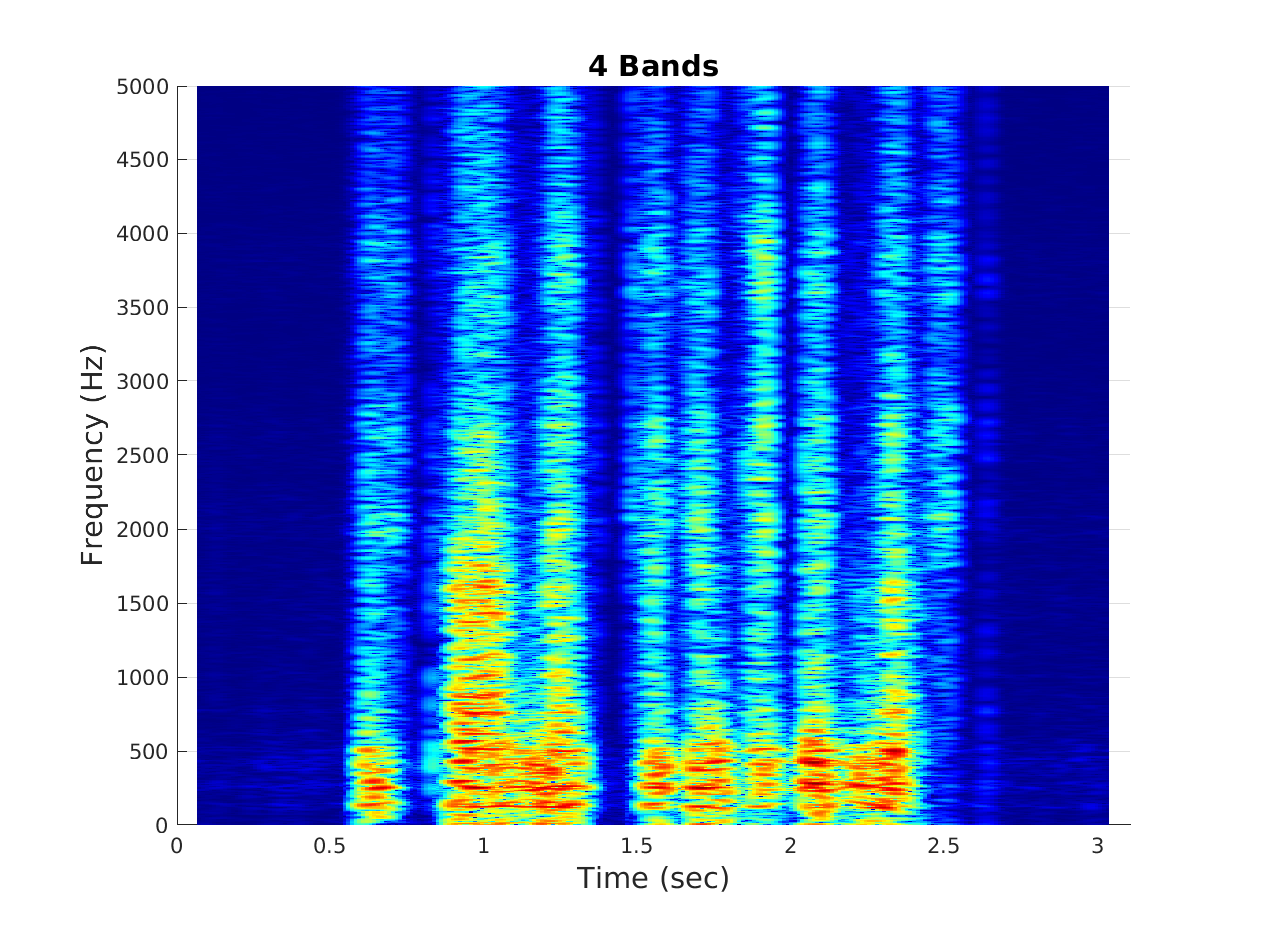
\includegraphics[width = .3\textwidth]{hilb_4} \\

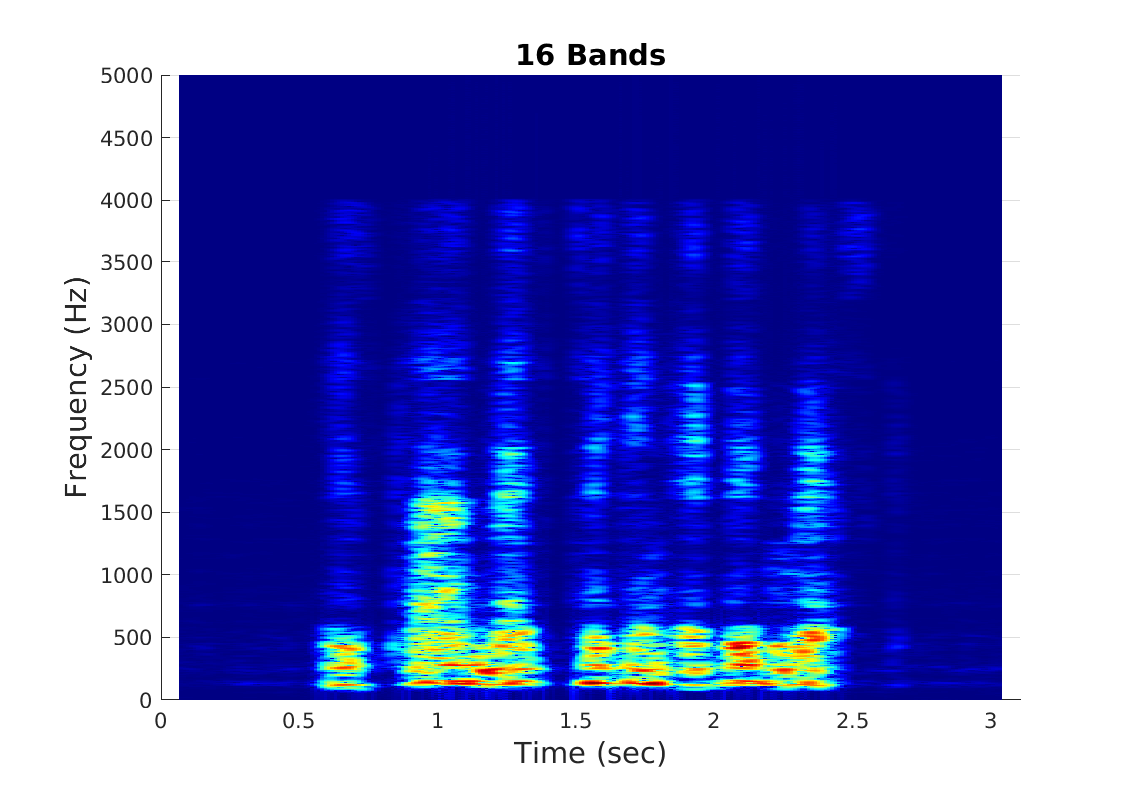
\includegraphics[width = .3\textwidth]{16_16}
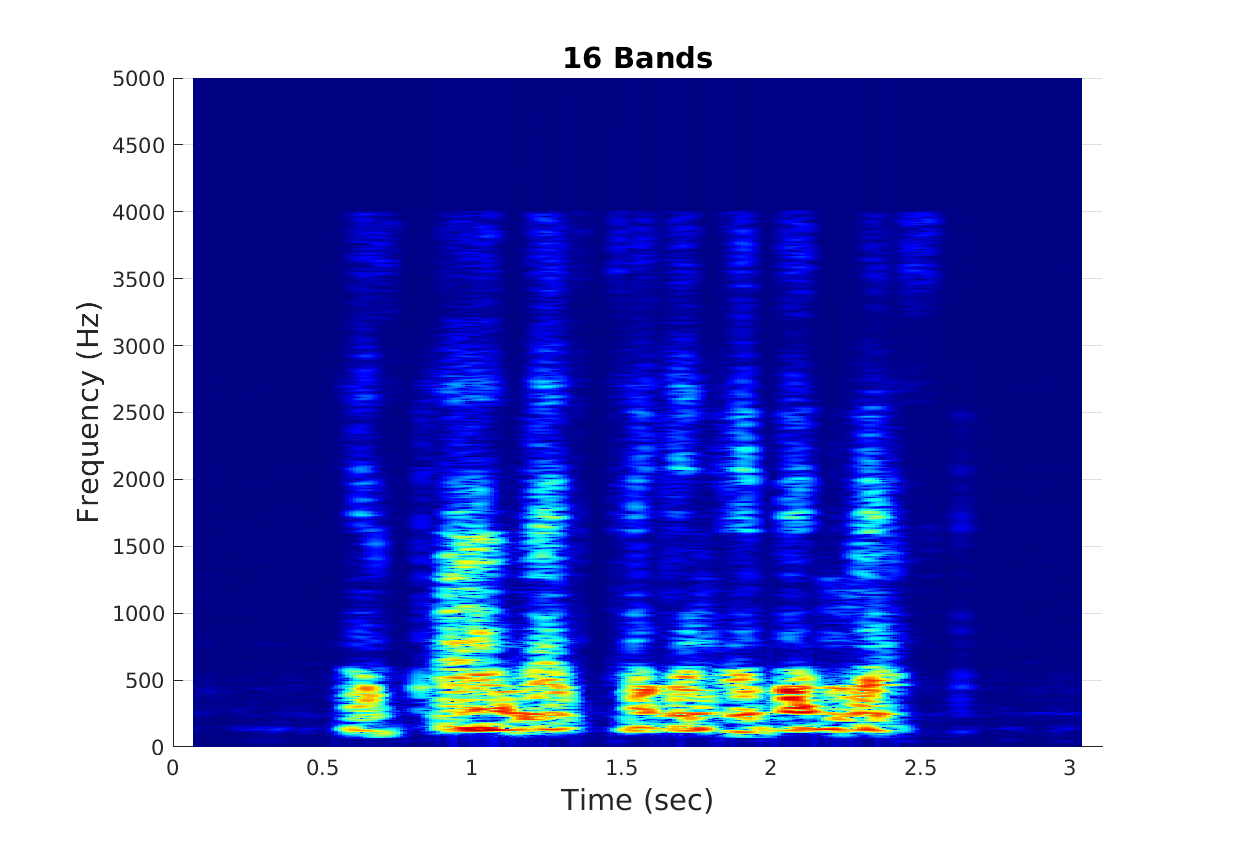
\includegraphics[width = .3\textwidth]{160_16}
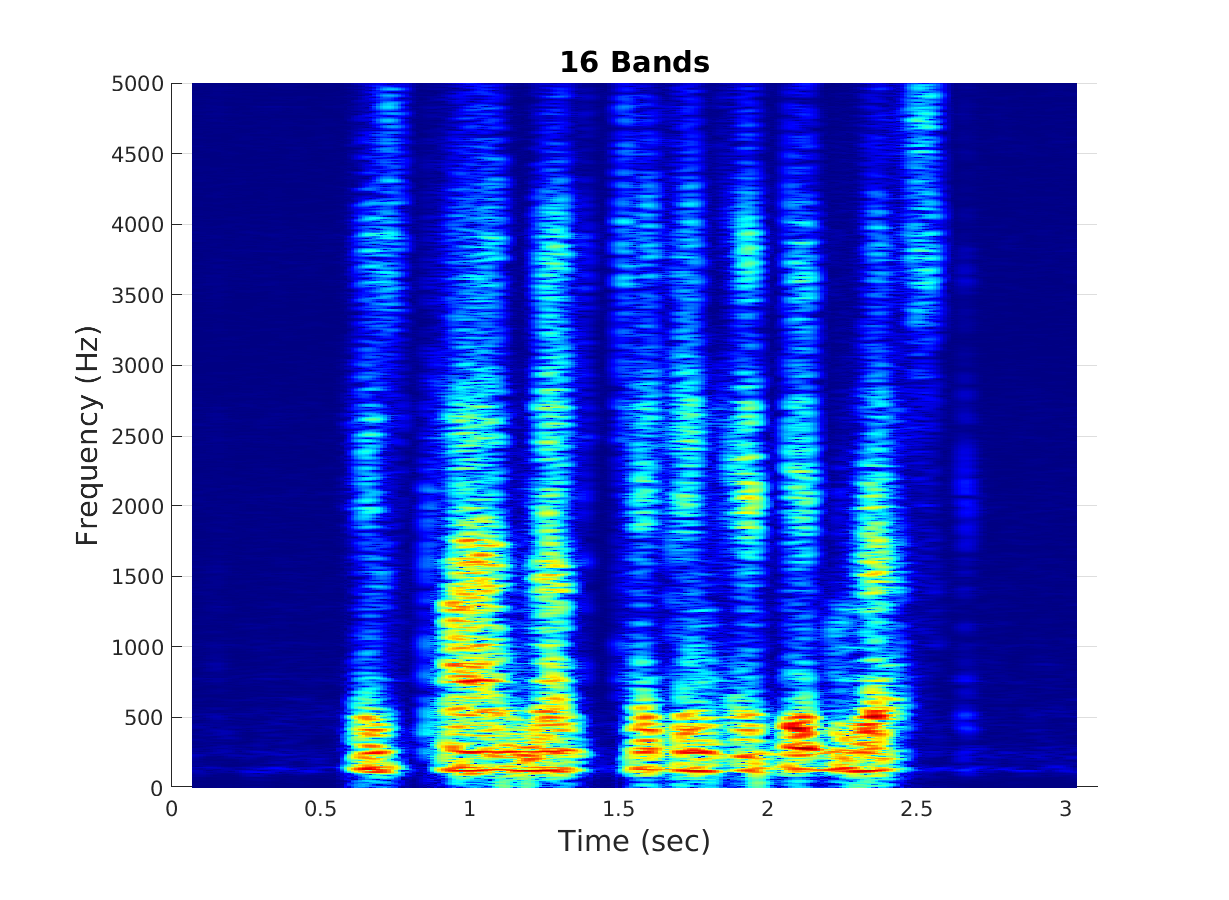
\includegraphics[width = .3\textwidth]{hilb_16} 
\end{center}

\newpage
The sharper cutoff at 4 kHz in the 16 and 160 Hz envelope extraction can be explained by the 4 kHz LPF filter I used  to emulate the Shannon et. al. (1995) study. Additionally, it is (again) clear that the Hilbert envelope extraction and presentation with a noise carrier captures more detail than the 16 and 160 Hz envelope extractions. All spectrograms tend to have closer representation of the raw recording as the number of bands increase.

\item The way we tested this was by taking ten of the SPIN-R sentences, and creating 16/160 Hz and Hilbert envelope extractions witha a spectrally matched noise carrier signal for all ten sentences using frequency bands [1,2,4,8,16]. Our code then randomly presented these stimuli and asked the user to guess which sentence was presented. We presented a total of 120 sentences/subject. We tracked correctness, in addition to reaction time. The code for this may be found in \verb|runTrialA.m|. Plots were made using \verb|compileData.m|. \\

From our results, it is evident that the Hilbert envelope allows for best representation of the sentence most-noticeably at the 1-2 Band filter-bank level. Above that, the 16/160 Hz envelope extraction works fairly well. It is important to consider the fact that our study was more primitive than the Shannon study, but demonstrated similar results. Instead of counting the number of words typed by the user, we went for a more simplistic approach to save time (10 alternative forced choice). Additionally, one of our subjects transcribed the sentences and de-bugged the code and was rather familiar with the 10 sentences that were used-- which likely resulted in better accuracy with sentence detection. The 16 Hz and 160 Hz envelope extractions resulted in very similar performance, though the 16 Hz extraction was slightly poorer.  \\

Our reaction time results were variable, but reaction time tends to decrease as number of bands increases. The Hilbert envelope extraction resulted in slightly lower reaction times on average, which also may demonstrate an increase in confidence of sentence identification as the number of bands increase. This was mainly just done out of curiosity.

\begin{center}
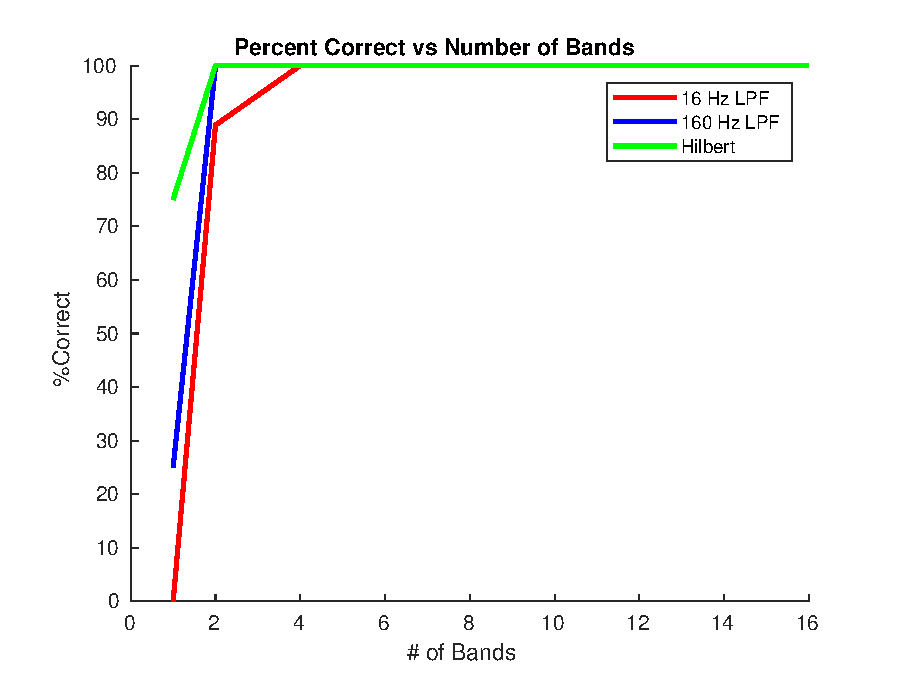
\includegraphics[width = .47\textwidth]{figA1}
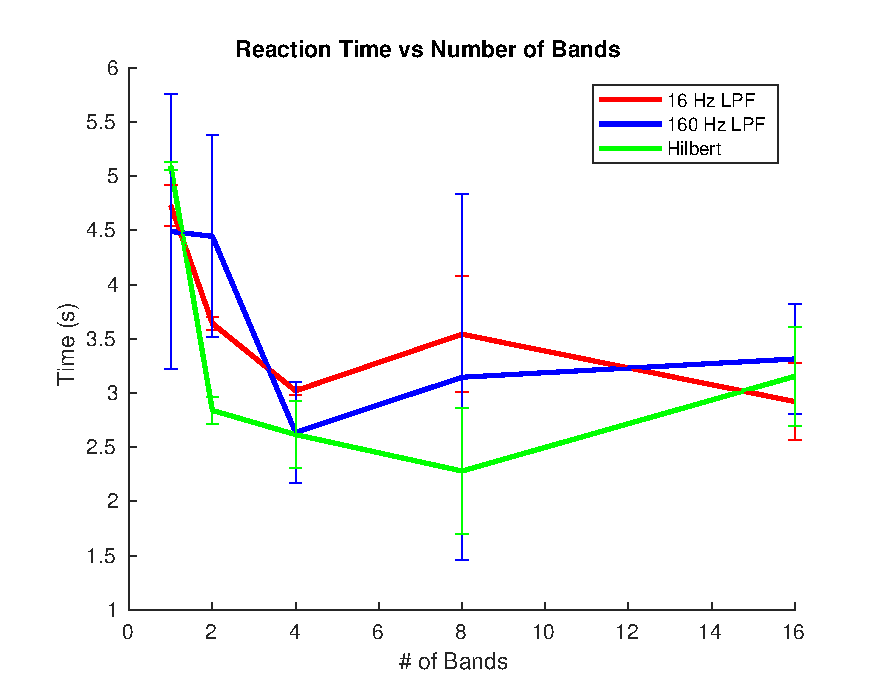
\includegraphics[width = .47\textwidth]{figA2}
\end{center}

\end{enumerate}


\section{Part B | Exploring potential for frequency modulation information to improve CI signal processing}

\begin{enumerate}[label = \alph*)]

\item The Delgutte implementation of acquiring the analytic signal is a smart approach because it prevents the computation of multiple large FFTs. Typically, the way the \verb|hilbert| function in Matlab works is by using a one-sided discrete-time frequency-domain approach outlined in a 1999 paper by Marple. While this method works well for obtaining an analytic signal, it would be computationally expensive in the chimera application because the code would have to first apply our band-pass filters to the signal, then send multiple time-domain signals to \verb|hilbert| which would do an FFT and inverse-FFT to return the analytic signal. \\

The Delgutte code combines a few steps into one very efficient method. The \verb|quad_filter_bank| function generates complex FIR filters \textit{in quadrature}. This means the filter coefficients from \verb|b| are in terms of $cos$ and $sin$ and where the $cos$ part is real and the $sin$ part is imaginary (and represents the Hilbert Transform). Since the analytic signal is in this form (since the Hilbert transform is a change in phase by $+\frac{\pi}{2}$ for neg. frequencies and $-\frac{\pi}{2}$ for pos. frequencies), the envelope and TFS information can be easily extracted by calculating the magnitude and phase angle of the filtered output, respectively (without having to use \verb|hilbert|). The chimera is then synthesized by multiplying the envelope from one signal by the TFS of another. The real part of \verb|b| simply represents the filter-bank bandpass filters, and can be used to refilter the chimera to compensate for filtering-related phase shifts-- as Delgutte does. \\

To create the noise carrier to make speech-noise chimeras, Delgutte uses \textit{spectrally-matched} noise. This means the noise carrier has the same frequency content as the speech signal. The way this is implemented is by taking an FFT of the speech signal, randomly changing the phase using $e^{2\pi j \omega_{random}}$, and taking the inverse FFT. 
%For long signals, the \verb|fftfilt| function used in the Delgutte code is more efficient than using the \verb|fft| and \verb|ifft| functions by themselves as \verb|hilbert| does, because it uses the \textit{overlap-add} method that breaks the computation into ``smaller pieces.'' \\

\item Our perceptual task consisted of asking the subject which sentence/music they heard most clear, using a single pair of chimeras (S1/S2, M1/M2). The code, found in \verb|runTrialB_music| or \verb|runTrialB_sentence|, noted if the subject chose the envelope or TFS. This was a 2 alternative forced choice study, and we presented 108 chimeras/subject for both sentences and music. Therefore, the TFS and ENV curves presented for each band are exactly inverse, unlike the Smith study, which asked subjects to identify multiple melodies/sentences if they heard them. The results are shown below (in green):

\begin{center} 
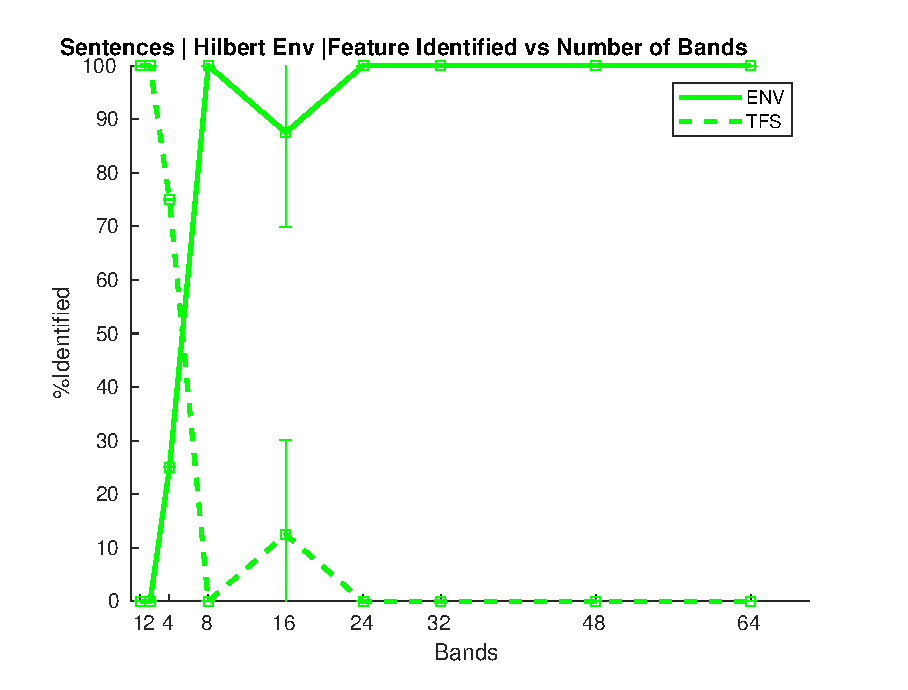
\includegraphics[width = .3\textwidth]{B1_3}
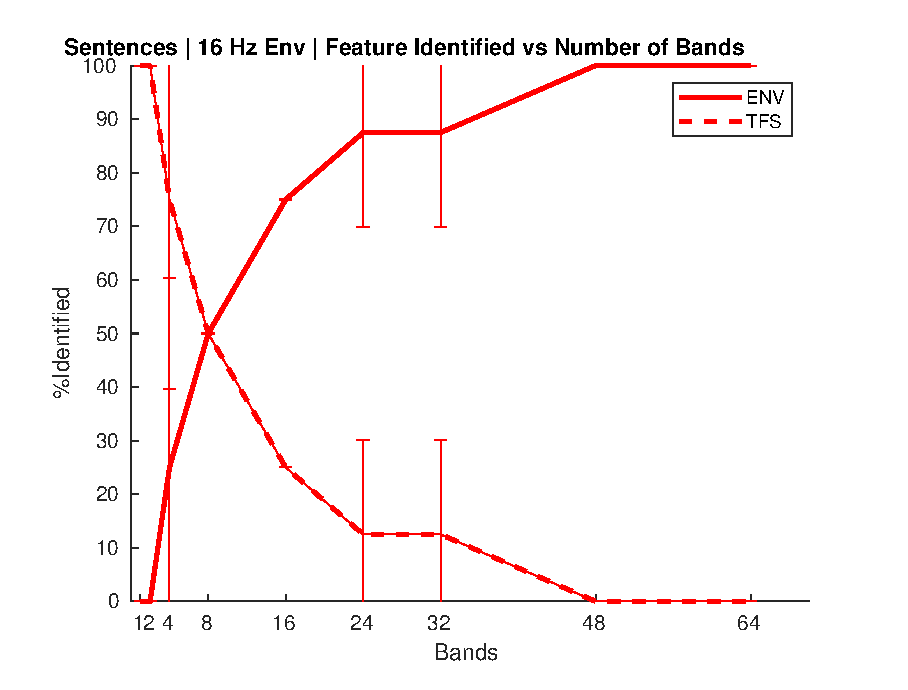
\includegraphics[width = .3\textwidth]{B1_1}
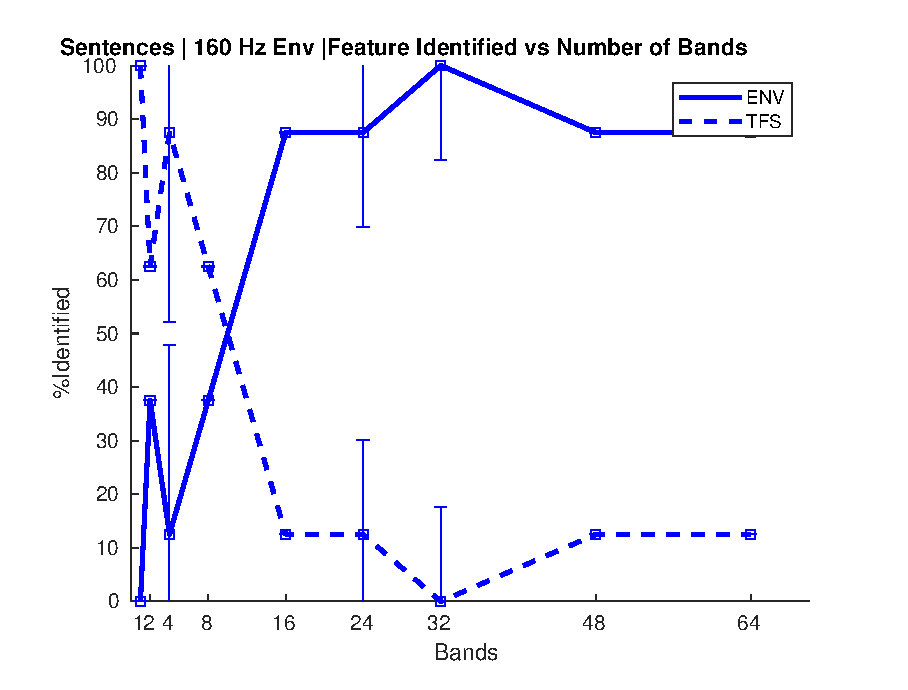
\includegraphics[width = .3\textwidth]{B1_2} \\

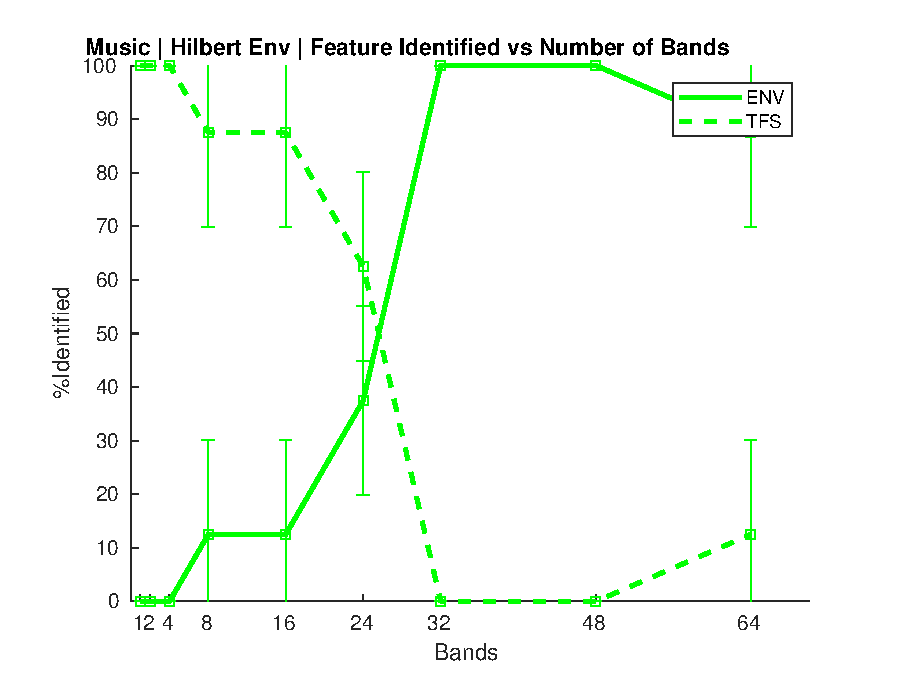
\includegraphics[width = .3\textwidth]{B2_3}
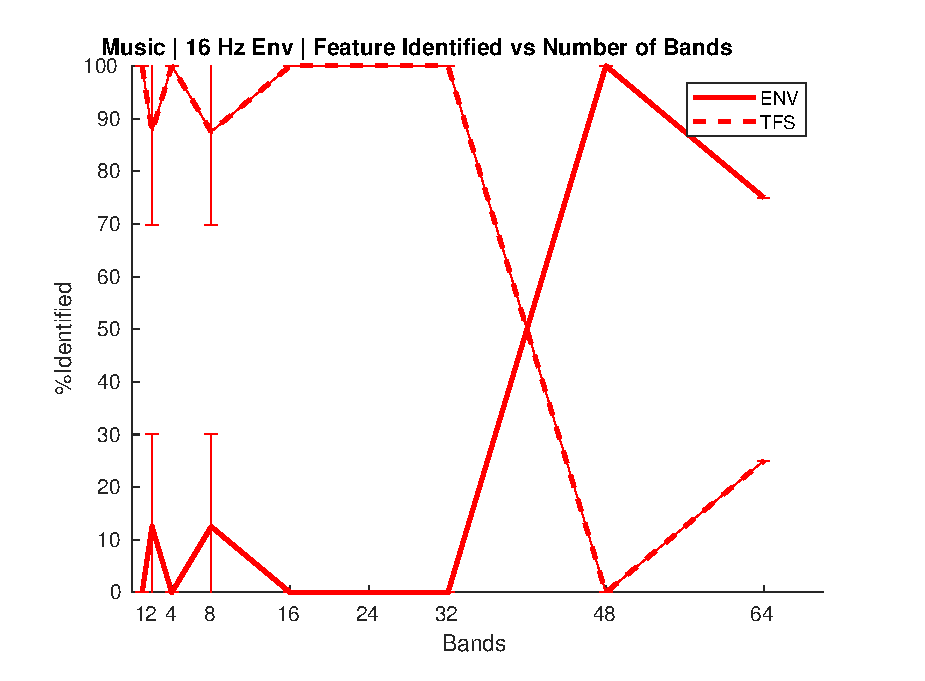
\includegraphics[width = .3\textwidth]{B2_1}
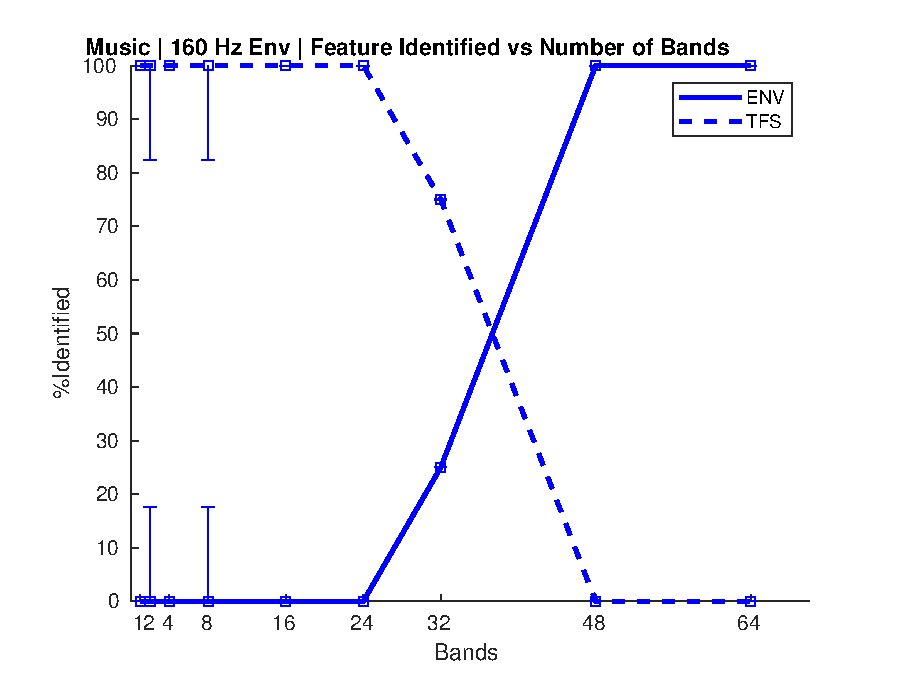
\includegraphics[width = .3\textwidth]{B2_2}

\end{center}

\item Using 16 Hz (red) and 160 Hz (blue) envelope extractions resulted in a slightly later crossing-over between the TFS and ENV compared to the Hilbert envelope extraction in both the sentence-sentence and music-music chimera trials. As mentioned in Part A, the Hilbert envelope extraction results in better representation of the fine changes in the signal envelope compared to the rectified low-pass filter approach. This may explain why the subjects, on average, identified hearing the envelope more clearly at lower bands in the Hilbert curves than they did in the 16 and 160 Hz curves.  

\item The main finding that is consistent between the Smith study and ours, despite our \textit{much} less extensive testing, is the general observation that the envelope of the waveform appears to be more useful in identifying words/speech patterns in sentences while the fine structure of the waveform seems to be more useful in identifying music. However, at very low numbers of bands, it appears fine structure is more important for sentence identification. In music, fine structure seems to be most useful at most frequency bands, until the transition at \textasciitilde 25-30 bands, where the envelope starts to become more useful.

\item Modern cochlear implants use a filter-bank paired with an envelope extraction approach similar to the methods we used in this project. Current implants transcode information in speech quite well, and give users the ability to succesfully listen and communicate. However, these implants do not transcode the temporal fine structure of sound because of the low-pass filtering or Hilbert transform used to derive the envelope for each band. This constraint is unfortunate, because in music, the temporal fine structure is important in conveying \textit{timbre}. Looking at the frequency spectrum of different instruments playing the same note shows small peaks beyond the fundamental frequency of that note. These small variations that exist in the TFS are what give instruments (and voices) their unique sounds, and are currently unable to be properly replicated by CIs. \\

Improving the ability of CI users to hear music or other sounds that have useful information in the TFS is a good next step in cochlear implant development. Most prospects for improving TFS delivery to CIs involve better replication of the TFS. One particular example is found in a 2012 study by Li et al. (Rubinstein Lab) that used a Harmonic Single Sideband Encoder (HSSE) to attempt to better convey TFS. The basic summary of this method is to identify and relay the harmonic content of a given signal to the output channels, which results in more TFS representation of a signal than methods such as continuous-interleaved-sampling (CIS). 
\end{enumerate}

\newpage
\section{Part C | Consiering a technical artifact with chimera synthesis and its potential implications} 

\begin{enumerate}[label = \alph*)]
\item The Zeng et al. (2004) paper makes a good point about envelope recovery from TFS. By using speech-noise and modulated speech-noise chimeras, Zheng observed that subjects were able to extract envelope information from TFS alone to a reasonable 40 \% accuracy when the TFS amplitudes were modulated randomly (using a noise envelope). He explained this as occurring because of the cochlea's ability (due to it's narrow-band nature) to recover envelope from TFS when broader bands are used in the filter-bank. Because of this, the author concludes that envelope is most important feature for speech recogntion, even at lower bands -- contrary to the data found in Fig. 2 of Smith (2009).\\

The authors' claim that envelope recovery is the most important feature for speech recognition at lower number of frequency bands was put to the test by both Gilbert et al. (2006) and Heinz et al. (2009), using perceptual and physiological measures, respectively. Gilbert used the Hilbert analytic signal to isolate the TFS of a vowel-consonant-vowel stimulus using multiple analysis bands [1,2,4,8,16], known as the HFS condition. Then, Gilbert computed a \textit{recovered envelope} by passing the HFS signals through a gammachirp auditory filter (presumably used to model the narrow-band nature of the cochlear filters), and again using the Hilbert analytic signal -- this time to extract the envelope. This output, known as the R-HFS condition, then represents a simulation of the envelope recovered by the cochlea from a signal's TFS alone. The authors then conducted a perceptual study, which showed that this R-HFS signal was enough to recover speech at \textasciitilde 1-4 bands, but at 8-16 bands, this effect appeared to be ``essentially abolished.''\\

Heinz et al. followed this work up with auditory nerve modeling and neurophysiology studies of the auditory nerve to further understand the context of the above findings in relation to auditory nerve firing. By looking at the spike trains from the nerve, more can be learned about what is happening in the auditory periphery free from the effects of behavior. The Heinz study used cross-correlation of spike trains observed in response to a speech signal envelope or TFS and those observed during its speech-noise chimeras. The authors found that the correlation between spike trains in response to the speech signal envelope and speech-TFS chimeras was significant for bands even up to 16, demonstrating that the envelope recovery effect may be even more significant than Gilbert et al. had initially thought.\\

This envelope recovery ``artifact'' may be the explanation behind the reversal of envelope/fine-time salience for the first two bands in Fig. 2 of the Smith study. Because the TFS at low bands results in a higher \textit{recovered envelope} (based on the findings from Gilbert and Zeng), it would appear from Fig. 2 that TFS is the responsible feature for speech recognition at low bands. In reality, this finding may be due to the \textit{recovered envelope} from the TFS, not the TFS itself. From the work by Heinz, it appears the \textit{recovered envelope} effect is relatively consistent from 1-16 band chimeras, so the effect may not be entirely due to the reasoning Zeng postulated, which implied it only occurs with a small number of frequency bands.

\item This artifact, if true, slightly affects the interpretation of Fig. 2 in the Smith study for 1 and 2-band chimeras for reasons mentioned above. Additionally, the findings from the Zeng, Gilbert, and Heinz studies may be incorrectly stretched to state that the reason TFS appears to be the more salient feature in music perception is due to envelope recovery by the cochlea. However, this is not accurate based on the spectral nature of the signals and the evidence that CI users struggle to enjoy music even when they are fully trained to understand speech. Feature extraction from speech is more related to the envelope, while the nuances and timbre that make music enjoyable occur in the fine structure. Therefore, Smith's conclusions about music perception likely remain accurate. \\

The envelope recovery ``artifact'' probably does not significantly affect the implications of Smith's study for today's CI processing, as most current CIs remove the TFS. If CIs were still 1-2 electrode devices, then the implications of this study may lead inventors to think TFS was the most important cue for speech recognition, when it actually may be the envelope recovery which is important in that case. However, according to the Heinz study, TFS envelope recovery still occurs even at higher numbers of frequency bands, which could be useful to take advantage of in future CIs that better replicate TFS. These future CIs would also likely improve music perception, as Smith's study implies.  
  
\end{enumerate}

\end{document}